\let\negmedspace\undefined
\let\negthickspace\undefined
\documentclass[journal]{IEEEtran}
\usepackage[a5paper, margin=10mm, onecolumn]{geometry}
%\usepackage{lmodern} 
\usepackage{tfrupee} 

\setlength{\headheight}{1cm} 
\setlength{\headsep}{0mm}     

\usepackage{gvv-book}
\usepackage{gvv}
\usepackage{cite}
\usepackage{amsmath,amssymb,amsfonts,amsthm}
\usepackage{algorithmic}
\usepackage{graphicx}
\usepackage{textcomp}
\usepackage{xcolor}
\usepackage{txfonts}
\usepackage{listings}
\usepackage{enumitem}
\usepackage{mathtools}
\usepackage{gensymb}
\usepackage{comment}
\usepackage[breaklinks=true]{hyperref}
\usepackage{tkz-euclide} 
\usepackage{listings}                                        
\def\inputGnumericTable{}                                 
\usepackage[latin1]{inputenc}                                
\usepackage{color}                                            
\usepackage{array}                                            
\usepackage{longtable}                                       
\usepackage{calc}                                             
\usepackage{multirow}                                         
\usepackage{hhline}                                           
\usepackage{ifthen}                                           
\usepackage{lscape}

\begin{document}

\bibliographystyle{IEEEtran}
\vspace{3cm}

\title{10.7.12}
\author{AI25BTECH11003 - Bhavesh Gaikwad}
{\let\newpage\relax\maketitle}

\renewcommand{\thefigure}{\theenumi}
\renewcommand{\thetable}{\theenumi}
\setlength{\intextsep}{10pt} 

\numberwithin{equation}{enumi}
\numberwithin{figure}{enumi}
\renewcommand{\thetable}{\theenumi}


\textbf{Question}: On the ellipse $4x^2 + 9y^2 = 1$, the points at which the tangents are parallel to the line $8x = 9y$ are\\

\hfill{(1999)}

\begin{itemize}
    \item[(a)] $(\frac{2}{5}, \frac{1}{5})$
    \item[(b)] $(\frac{-2}{5},\frac{1}{5})$
    \item[(c)] $(\frac{-2}{5},\frac{-1}{5})$
    \item[(d)] $(\frac{2}{5},\frac{-1}{5})$
\end{itemize}

\bigskip
 
\textbf{Solution:}\\
Given: Ellipse: $4x^2 + 9y^2 = 1$ \& Line: $8x-9y=0$\\

Parameters of Ellipse:
\begin{equation}
\vec{V} = \myvec{4/9 & 0 \\ 0 & 1}, \, \vec{u} = \myvec{0 \\ 0}, \, e = \dfrac{\sqrt{5}}{3}, \, \vec{n} = \myvec{1 \\ 0}, \, f = \frac{-1}{9}
\end{equation}

Equation of Ellipse:
\begin{equation}
    \vec{X}^\top \myvec{4/9 & 0 \\ 0 & 1}\vec{X} = \frac{1}{9}
\end{equation}

Parameters of Given Line:
\begin{equation}
\vec{m} =  \myvec{8 \\ -9}, \, \vec{h}=\myvec{0 \\ 0}
\end{equation}

Equation of Given Line:
\begin{equation}
     L: \, \vec{X} = k\vec{m} \text{  OR  } L: \, \vec{X} = k\myvec{8 \\ -9}
\end{equation}

Since, Tangents are parallel to L,
\begin{equation}
    \therefore \text{The normal vector to the tangents is } \vec{n}_2 = \myvec{9 \\ 8}
\end{equation}

Let $\vec{q}_i$ be the points of contact. i =1,2.
\begin{equation}
    \vec{q}_i = \vec{V}^{-1}(k_i\vec{n}_2 - u) \qquad
    \text{where, } k_i = \pm \sqrt{\dfrac{f_o}{\vec{n}_2^\top \vec{V}^{-1} \vec{n}_2}}
\end{equation}

\begin{equation}
    f_o = \vec{u}^\top\vec{V}^{-1}\vec{u} - f = 1/9
\end{equation}

From Equation 0.6,
\begin{equation}
    \vec{q}_1 = \myvec{\dfrac{-2}{5} \\\\ \dfrac{1}{5}} \qquad \& \qquad \vec{q}_2 = \myvec{\dfrac{2}{5} \\\\ \dfrac{-1}{5}}
\end{equation}


\begin{align*}
    \boxed{\text{Thus, Option B and D are correct.}}
\end{align*}



\begin{figure}[htbp]
    \centering
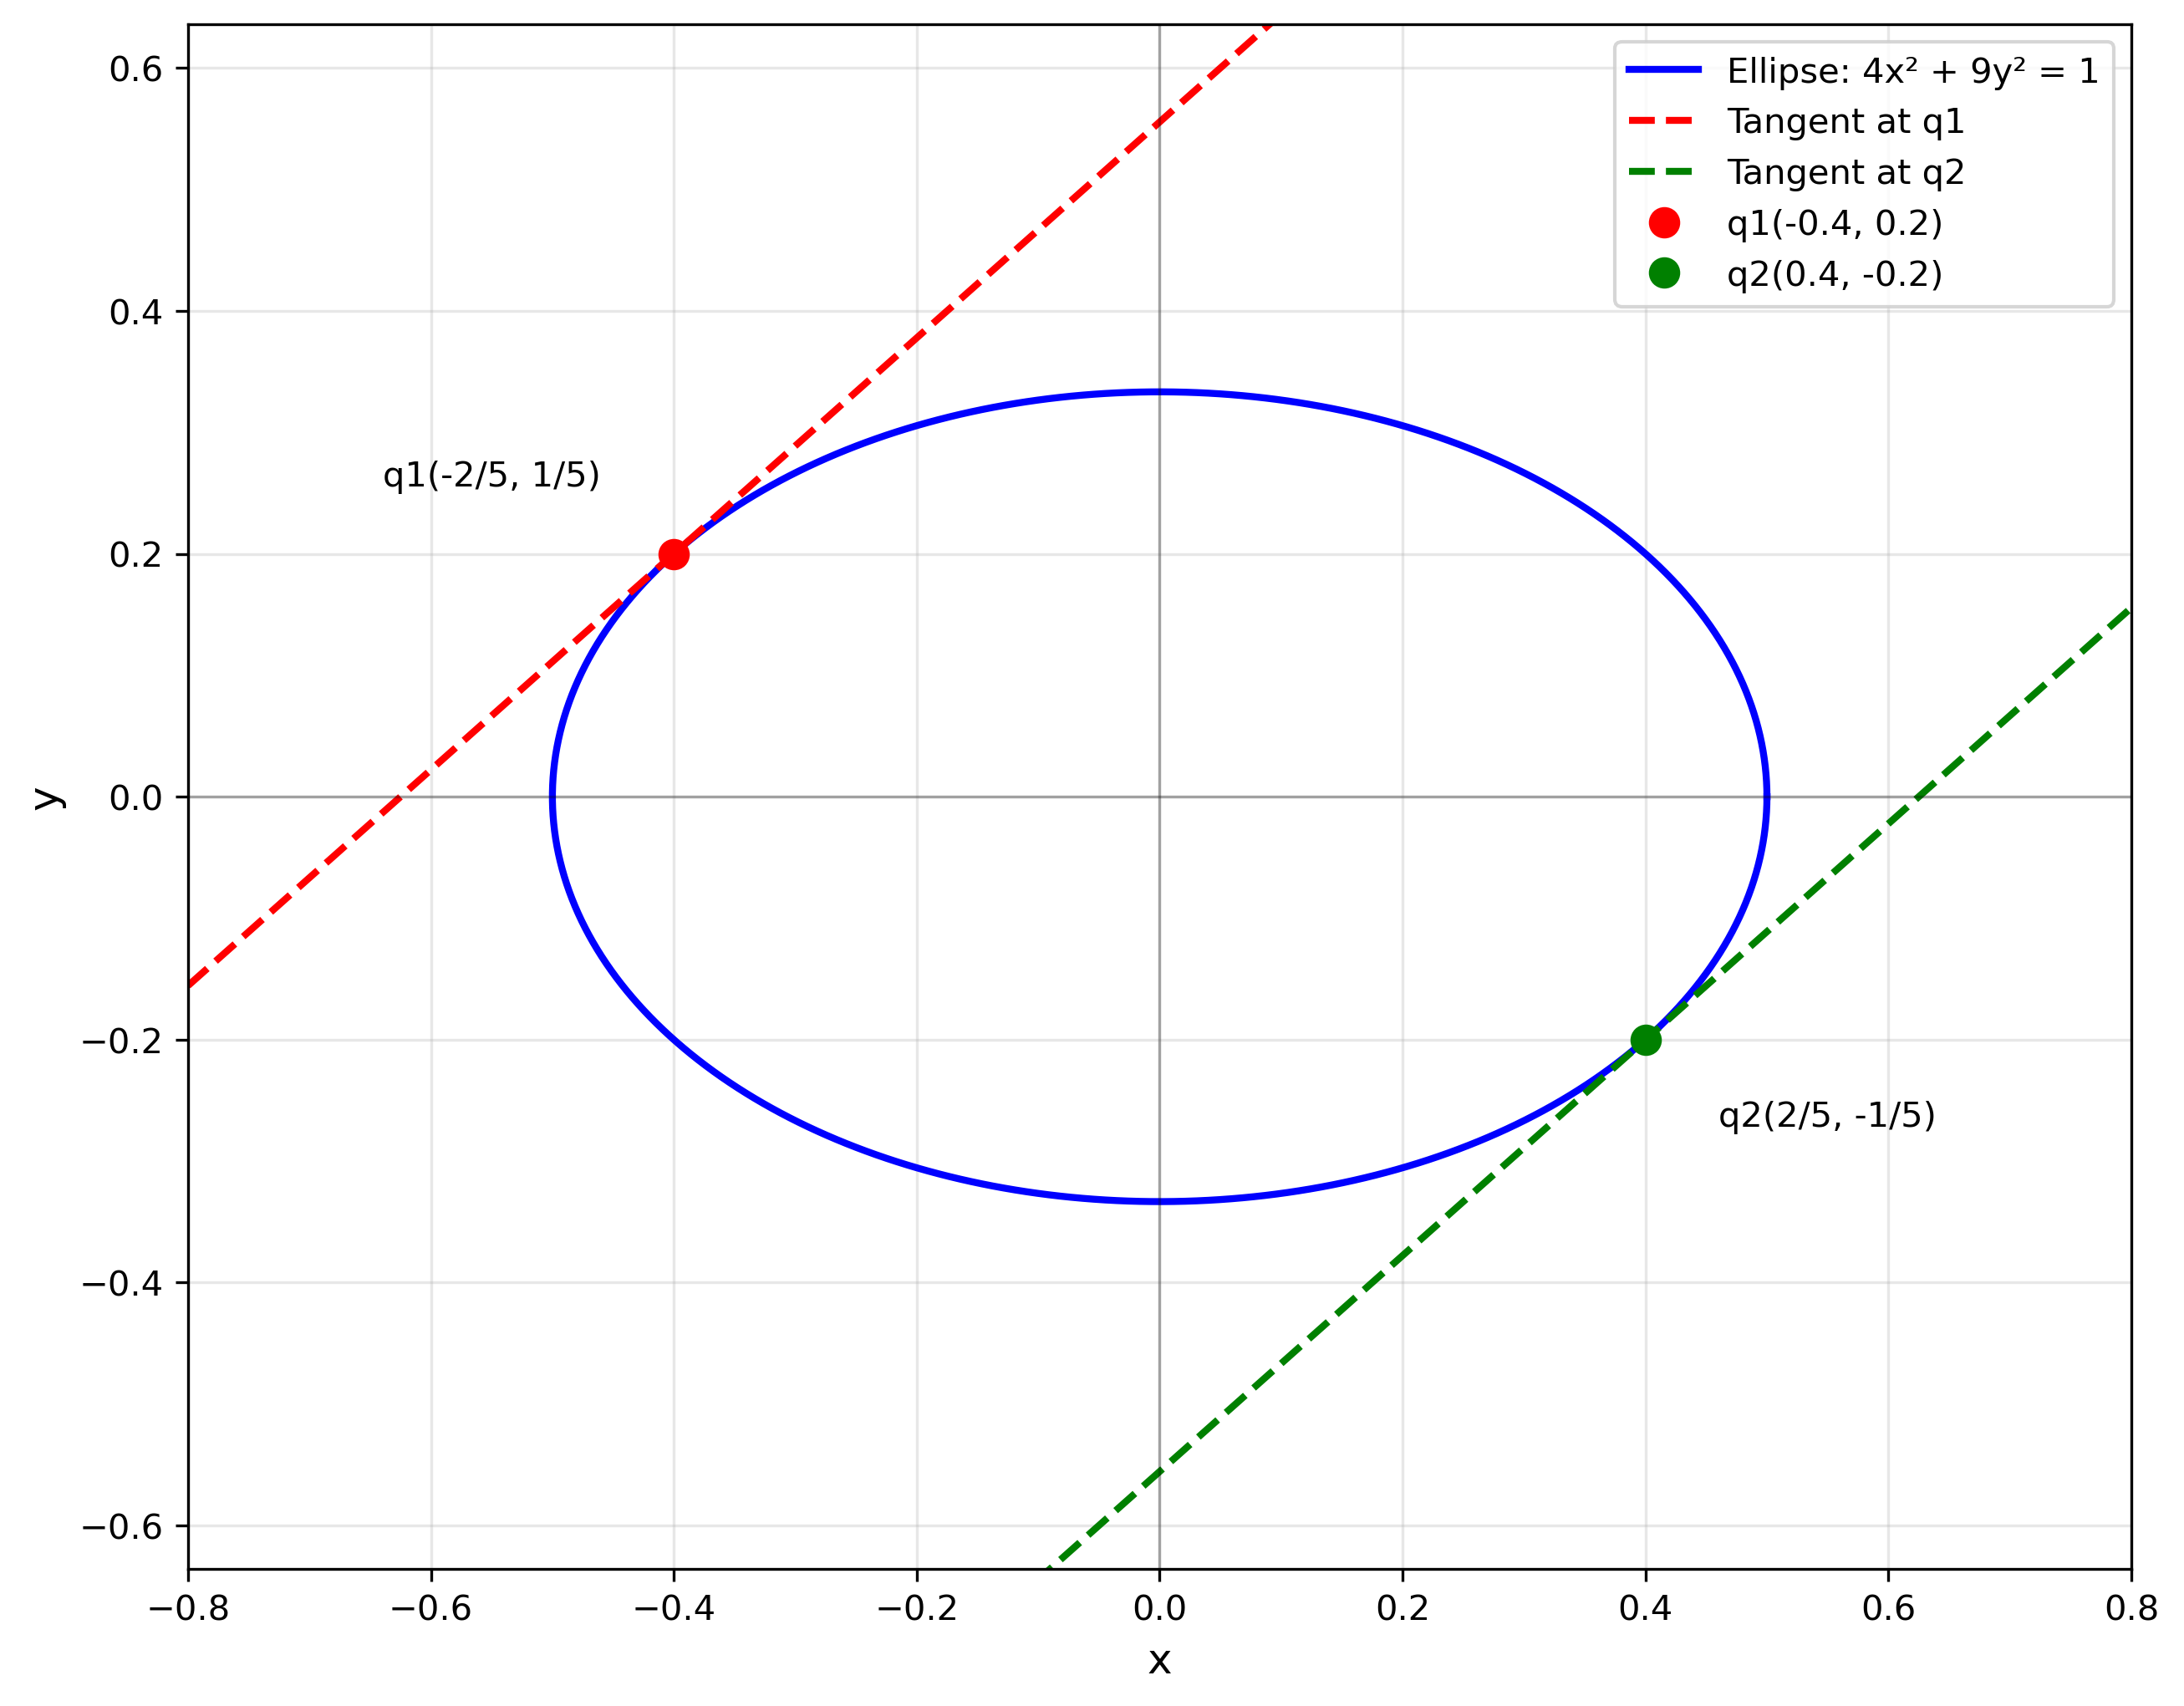
\includegraphics[width=\columnwidth]{figs/fig1.png}
    \caption{}
    \label{fig:figs/fig1.png}
\end{figure}

\end{document}  
